\documentclass[letterpaper, 11pt]{article}

\usepackage{jheppub}
\usepackage{bm}
\usepackage{graphicx}
\usepackage{epstopdf}
\usepackage{amsmath, amssymb}

\usepackage{amsfonts,amssymb,epsfig,amsmath,mathtools,tabu}
\usepackage{verbatim,booktabs}

%\usepackage[utf8]{inputenc}
%\usepackage{textcomp,setspace}
\usepackage[inline]{enumitem}

\usepackage{hyperref,caption,subcaption}
\usepackage{xcolor,tikz,graphicx,afterpage}
\usetikzlibrary{shapes.geometric,positioning}
%\usetikzlibrary{cd}


\newcommand{\be}{\begin{eqnarray}}
\newcommand{\ee}{\end{eqnarray}}
\newcommand{\nn}{\nonumber}
\newcommand{\bn}{\begin{enumerate}}
\newcommand{\en}{\end{enumerate}}

%%%%%%%%%%%%%%%%%%% Figures %%%%%%%%%%%%%%%%%%%%%%%%%%%

\newcommand{\fig}[3]{
\begin{figure}
\centerline{\epsfxsize=#1\epsfbox{#2.eps}}
\newcaption{#3. \label{#2}}
\end{figure}
}

%%%%%%%%%%%%% Double line letters using amssymb %%%%%%%%%%%%%%%%

\def\identity{{\rlap{1} \hskip 1.6pt \hbox{1}}}
\def\iden{\identity}

\def\IB{\mathbb{B}}
\def\IC{\mathbb{C}}
\def\ID{\mathbb{D}}
\def\IH{\mathbb{H}}
\def\IM{\mathbb{M}}
\def\IN{\mathbb{N}}
\def\IP{\mathbb{P}}
\def\IR{\mathbb{R}}
\def\IZ{\mathbb{Z}}

%%%%%%%%%%%%%%%% Caligraphic letters %%%%%%%%%%%%%%%%%%

\def\CA{{\cal A}}
\def\CB{{\cal B}}
\def\CC{{\cal C}}
\def\CD{{\cal D}}
\def\CE{{\cal E}}
\def\CF{{\cal F}}
\def\CG{{\cal G}}
\def\CH{{\cal H}}
\def\CI{{\cal I}}
\def\CJ{{\cal J}}
\def\CK{{\cal K}}
\def\CL{{\cal L}}
\def\CM{{\cal M}}
\def\CN{{\cal N}}
\def\CO{{\cal O}}
\def\CP{{\cal P}}
\def\CQ{{\cal Q}}
\def\CR{{\cal R}}
\def\CS{{\cal S}}
\def\CT{{\cal T}}
\def\CU{{\cal U}}
\def\CV{{\cal V}}
\def\CW{{\cal W}}
\def\CX{{\cal X}}
\def\CY{{\cal Y}}
\def\CZ{{\cal Z}}

%%%%%%%%%%%%%%%%%% Greek letters %%%%%%%%%%%%%%%%%%%%%%%%%%%%

\def\a{\alpha}
\def\b{\beta}
\def\g{\gamma}
\def\d{\delta}
\def\e{\epsilon}
\def\ve{\varepsilon}
\def\z{\zeta}
% eta
\def\th{\theta}
\def\vth{\vartheta}
\def\i{\iota}
\def\k{\kappa}
\def\l{\lambda}
\def\m{\mu}
\def\n{\nu}
% xi
% o
% pi
\def\vp{\varpi}
\def\r{\rho}
\def\vr{\varrho}
\def\s{\sigma}
\def\vs{\varsigma}
\def\t{\tau}
\def\u{\upsilon}
% phi
\def\vph{\varphi}
% chi
\def\ch{\chi}
% psi
\def\w{\omega}
%
\def\G{\Gamma}
\def\D{\Delta}
\def\Th{\Theta}
\def\L{\Lambda}
% Xi
% Pi
\def\S{\Sigma}
\def\Y{\Upsilon}
% Phi
% Psi
\def\O{\Omega}


%%%%%%%%%%%%%%%%% Mathematical Symbols %%%%%%%%%%%%%%%%%%%%%%%%%%%%

\def\half{\frac{1}{2}}
\def\thalf{{\textstyle \frac{1}{2}}}
\def\imp{\Longrightarrow}
\def\goto{\rightarrow}
\def\para{\parallel}
\def\vev#1{\langle #1 \rangle}
\def\del{\nabla}
\def\grad{\nabla}
\def\curl{\nabla\times}
\def\div{\nabla\cdot}
\def\p{\partial}
\newcommand{\bra}[1]{\langle{#1}|}
\newcommand{\ket}[1]{|{#1}\rangle}
\def\fslash{\displaystyle{\not}}

%%%%%%%%%%%%%%%%%%%% Normal font in math %%%%%%%%%%%%%%%%%%%%%%%%%%

\def\Tr{{\rm Tr}}
\def\tr{{\rm tr}}
\def\det{{\rm det}}



%%%%%%%%%%%%%%%%%%%%%%%%%%%%%%%%%%%%%%%%%%%%%%%%%%%%%
\title{Instantons from Blow-up}

\author[a]{Joonho Kim,}
\author[b]{Sung-Soo Kim,}
\author[c]{Ki-Hong Lee,}
\author[a]{Kimyeong Lee,}
\author[a]{and Jaewon Song}
\affiliation[a]{School of Physics, Korea Institute for Advanced Study, Seoul 02455, Korea}
\affiliation[b]{School of Physics, University of Electronic Science and Technology of China,\\ No.4, Section 2, North Jianshe Road, Chengdu, Sichuan 610054, China}
\affiliation[c]{Department of Physics and Astronomy \& Center for Theoretical Physics\\ Seoul National University, Seoul 08826, Korea}
\emailAdd{joonhokim@kias.re.kr}
\emailAdd{sungsoo.kim@uestc.edu.cn}
\emailAdd{khlee11812@gmail.com}
\emailAdd{klee@kias.re.kr}
\emailAdd{jsong@kias.re.kr}

\abstract{
The Nekrasov partition function for 4d $\CN=2$ or 5d $\CN=1$ gauge theory on the blow up of a point $\hat{\IC}^2$ can be written in terms of the partition function on the flat space $\IC^2$. At the same time, the partition function on the blow up is identical to the partition function on a flat space for sufficiently large class of examples. 
This relation enables us to compute the instanton partition functions for 4d $\CN=2$ and 5d $\CN=1$ gauge theories for arbitrary gauge theory with large class of matter representations without knowing explicit construction of the instanton moduli space. Remarkably, the instanton partition function is completely determined by the perturbative part. 
We obtain the partition function for the previously unknown theories: exceptional gauge groups $EFG$ with fundamental/spinor hypermultiplets and more. We also compute the case with $SU(6)$ with rank-3 antisymmetric tensor and compare with the topological vertex computation using the recently found 5-brane web configuration. 
}


\preprint{KIAS-P19???, SNUTP19-???}

%%%%%%%%%%%%%%%%%%%%%%%%%%%%%%%%%%%%%%%%%%%%%%%%%%%
\begin{document}
\maketitle

\section{Introduction} \label{sec:intro}


The Seiberg-Witten prepotential provides a complete description for the low energy dynamics of 4d $\mathcal{N}=2$ or 5d $\mathcal{N}=1$ gauge theory in its Coulomb branch \cite{Seiberg:1994rs,Seiberg:1994aj}. It is a polynomial in the VEV of the vector multiplet scalar that parameterizes the Coulomb branch moduli space. Quantum correction to the prepotential is known to be one-loop exact, while there also exist non-perturbative corrections coming from Yang-Mills instantons. 

An efficient way to compute the fully quantum corrected prepotential $\mathcal{F}$ is to study the Nekrasov partition function $\mathcal{Z}$ on $\Omega$-deformed $\mathbb{C}^2$ or $\mathbb{C}^2 \times S^1$, i.e., $\mathcal{F} = \lim_{\epsilon_{i}\rightarrow 0} \epsilon_1 \epsilon_2 \log{\mathcal{Z}}$ \cite{Nekrasov:2002qd,Nekrasov:2003rj,Nakajima:2003pg}.
It can be written as the product of the classical, one-loop, and instanton contributions,
\begin{align}
  \mathcal{Z}(\vec{a}, \vec{\mathfrak{m}}, \e_1, \e_2, \mathfrak{q}) = \mathcal{Z}_{\textrm{class}}(\vec{a}, \e_1, \e_2, \mathfrak{q}) \ \mathcal{Z}_{\textrm{1-loop}} (\vec{a}, \vec{\mathfrak{m}}, \e_1, \e_2) \ \mathcal{Z}_{\textrm{inst}}(\vec{a}, \vec{\mathfrak{m}}, \e_1, \e_2, \mathfrak{q}),
\end{align}
where the instanton piece is the fugacity sum over all multi-instanton contributions:
\begin{align}
  \mathcal{Z}_{\textrm{inst}}(\vec{a}, \vec{\mathfrak{m}}, \e_1, \e_2, \mathfrak{q}) = 1 + \sum_{k=1}^\infty \mathfrak{q}^k \mathcal{Z}_k(\vec{a}, \vec{\mathfrak{m}}, \e_1, \e_2).
\end{align}
The instanton part of the partition function in the $\Omega$-background can be computed once we know appropriate instanton moduli space. For the classical gauge group, the ADHM construction of the moduli space provides a direct way compute the instanton partition function. The ADHM construction can be understood as the quantum mechanics described by the Dp-D(p+4) system. The Higgs branch moduli space of the Dp system gives the desired moduli space. Matter fields can be also introduced by considering the world-volume theory on the D0-branes of the D0-D4-D8 system. 

But there is no ADHM type construction for the exceptional gauge groups or generic type of matter fields. String-theoretic picture implies that they require strong-coupling dynamics or non-Lagrangian field theories to realize instanton moduli space of exceptional group as a vacuum moduli space. There has been a few results regarding the exceptional instantons. 

In this paper, we generalize the approach of \cite{Keller:2012da} where the instanton partition function was obtained via blow-up formula of Nakajima-Yoshioka \cite{Nakajima:2003pg,Nakajima:2003uh,Nakajima:2005fg} for the pure YM theory. We propose a general blow-up formula for general gauge theory with arbitrary representations, under the condition that the matter representation is not too large. This enables us to compute the instanton partition function for a numerous gauge theories that has not been known before, without relying on to the explicit construction of the moduli space. 

The basic idea is as follows: Let us consider a one-point blow up $\hat{\IC^2}$ of the flat space $\IC^2$. The \emph{full} partition function on $\hat{\IC^2}$ can be written in terms of the products of the \emph{full} partition function of $\IC^2$. But at the same time, the partition function on the blowup is identical to that of the flat space since we can smoothly blow-down $\hat{\IC^2}$ to $\IC^2$.\footnote{As long as the matter representation is not `too large'.} This provides us a functional relation for the partition function, which turns out to be enough to determine the instanton partition function itself. Remarkably, this relation is completely determined by the perturbative part of the partition function. Therefore we arrive at a surprising conclusion: The \emph{perturbative} physics determine the \emph{non-perturbative} physics! 




\paragraph{Notation}
The equivariant parameters $\epsilon_{1}, \epsilon_2, \vec{a}$ are associated to the $U(1)^2 \times U(1)^{|G|}$ action on the $k$-instanton moduli space $\mathcal{M}_{k,G}$. Additional parameters $\vec{\mathfrak{m}}$ are introduced if the gauge theory has an extra  flavor symmetry. The instanton fugacity $\mathfrak{q}$ can be written as $\mathfrak{q}\equiv\Lambda^{b_0}$ (4d) or $\mathfrak{q}\equiv \exp(2\pi i \Lambda)$ (5d) where $\Lambda$ denotes the bare coupling of the 4d/5d gauge theory.

Throughout Section~\ref{sec:blowup}, we will characterize the partition function in terms of $m_i \equiv \mathfrak{m}_i + \epsilon_+$ (where $\epsilon_+ \equiv \frac{\epsilon_1 + \epsilon_2}{2}$) as a reflection of the Donaldson-Witten twist by $SU(2)_R$ symmetry. Here $m_i$ corresponds to the `physical' mass parameter of a matter hypermultiplet. We will also stick to the `effective' instanton fugacity $q \equiv \mathfrak{q} e^{{b_0}\epsilon_+}$, which absorbs the $SU(2)_R$ generated mass of fermionic instanton zero modes, in describing the 5d Nekrasov partition function.

%%%%%%%%%%%%%%%%%%%%%%%%%%%%%%%%%%%%%%%%%%%%%%%%%%%%%%%%%%%%%%%%

\section{Instanton Counting from Blow-up} \label{sec:blowup}



The essential idea of using the blow-up of ${\IC}^2$ for instanton counting is that the gauge theory partition function for a 4d $\CN=2$ (or 5d $\CN=1$) theory on a blow up of a point $\hat{\IC}^2$ (or $S^1 \times \hat{\IC}^2$) can be written in two different ways. This allows us to write a recursion relation for the instanton partiton function that can be solved easily \cite{Nakajima:2003pg, Nakajima:2003uh,Nakajima:2005fg, Keller:2012da}. 






\paragraph{Partition function on the Blow-up $\hat{\IC}^2$}

One of the expressions for the partition function $\hat{\mathcal{Z}}$ on the blow-up $\hat{\IC}^2$ comes from the Coulomb branch localization, which results that $\hat{\mathcal{Z}}$ can be obtained by patching together the flat-space partition functions \cite{Nekrasov:2003vi}.


 The blow-up of a point in $\IC^2$ can be described as a subspace of $\IC^2 \times \IP^1$, defined as
\begin{align}
 \{ (x, y), [z: w] \in \IC^2 \times \IP^1 | xw = yz \} \ , 
\end{align}
where $[z:w]$ represents the homogeneous coordinates on $\IP^1$. Notice that this space is identical to $\IC^2$ when $(x, y) \neq (0, 0)$, and the origin is replaced by complex projective plane. We will be considering the $U(1)^2$-equivariant partition function, with each $U(1)$'s acting as the rotation of a complex plane. This $U(1)^2$ action acts on $\hat{\IC}^2$ as
\begin{align}
 ((x, y), [z: w]) \mapsto (e^{i \e_1} x, e^{i \e_2} y), [e^{i \e_1} z, e^{i \e_2} w]) \ . 
\end{align}
The zero sized instantons will be located at two fixed points of the $U(1)^2$ action, namely the north and south pole of the $\mathbb{P}^1$. At these points, the weights of the $U(1)^2$ action become
\begin{align}
 ((0, 0), [1, 0]) : (\e_1, \e_2 - \e_1) , \qquad ((0, 0), [0, 1]): (\e_1 - \e_2, \e_2) \ . 
\end{align}

The full partition function $\hat{Z}$ on $\hat{\IC}^2$, which includes both the perturbative and instanton contributions, can be written as a sum over the product of the partition functions at two fixed points \cite{Nekrasov:2003vi, Gottsche:2006bm, Gottsche:2006tn, Gasparim:2008ri, Bonelli:2012ny}. Here we turn off any external flux that can be supported on the $\IP^1$. Then 
\begin{align} \label{eq:blowup}
 \hat{Z}(\vec{a}, \e_1, \e_2) = \sum_{\vec{k} \in \Lambda} Z(\vec{a}+ \vec{k} \e_1, \e_1, \e_2 - \e_1) Z(\vec{a}+\vec{k} \e_2, \e_1 - \e_2, \e_2) \ , 
\end{align}
% where $Z(\vec{a}, \e_1, \e_2)$ is the full partition function on $\IC^2$ where $\vec{a}$ is the Coulomb VEV parameter. 
where the sum is taken over the coweight lattice $\Lambda$  of the gauge group.
This expression is obtained by performing the localization on the Coulomb branch. On the Coulomb branch, the gauge group is broken to $U(1)^r$ where $r$ is the rank of the gauge group. We need to patch together all possible field configurations with zero sized instantons located at the north and south poles.  All the inequivalent configurations are labeled by the vector $\vec{k}$ of the first Chern numbers, corresponding to different flux configurations on the divisor $\mathbb{P}^1$. The shift of the Coulomb parameter is due to the following reason \cite{Bershtein:2015xfa}: At a fixed point $p$, the $U(1)^r$ vector multiplet scalar $\vec{\Phi}$ takes the value of $\vec{a} + \vec{k}H|_p$, where $H$ is the moment map for the $U(1)^2$ action $V$ on the K\"ahler 2-form $\omega$, i.e., $\iota_V \omega = dH$. One can find $H|_{N} = \epsilon_1$ and $H|_{S} = \epsilon_2$ as 
\begin{align}
  \label{eq:moment-map}
  H = 
  \begin{dcases}
     \frac{\epsilon_1|z|^2+ (\epsilon_2 - \epsilon_1)|w|^2}{|z|^2+|w|^2} & \text{(around the north pole)},\\
   \frac{(\epsilon_1-\epsilon_2)|z|^2+ \epsilon_2|w|^2}{|z|^2+|w|^2} & \text{(around the south pole)}.
  \end{dcases}
\end{align}

\paragraph{Partition function on $\hat{\IC^2}$ vs $\IC^2$}
Alternatively, it is  known that the partition function $\hat{\CZ}$ on the blow-up $\hat{\IC}^2$ ($S^1 \times \hat{\IC^2}$) is actually identical to the flat space partition function $\CZ$  \cite{Nakajima:2003pg, Nakajima:2003uh,Nakajima:2005fg}.
 
This can be argued as follows: The blow-up $\hat{\IC}^2$ is identical to $\IC^2$ except for the origin, which is replaced by the exceptional divisor $\IP^1$. It can also be  identified as the total space of the bundle $\CO(-1) \to \IP^1$. 
The Nekrasov partition function gets contributions only from the zero-size instantons localized at the fixed points of the $U(1)^2$ action, thus the size of the divisor should not affect the partition function as we smoothly shrink it. Therefore, we expect that the partition function on the blow-up to be identical to that of the flat $\IC^2$ (or $\IC^2 \times S^1$).

This is a special feature of the blow-up of a point. In principle, there can be extra states coming from the $\IP^1$. As we shrink the size of the $\IP^1$, there may appear extra massless states which can contribute to the partition function. This happens when there is a singularity as we blow down the $\IP^1$. 
For example, if we consider the total space of $\CO(-2) \to \IP^1$ and shrink the base, we land on the orbifold $\IC^2/\IZ_2$ which is singular at the origin. However, in our case, we do not obtain any singularity as we blow down the sphere. \textcolor{red}{We will discuss later that this simple picture does not necessarily hold when there are too many hypermultiplets. But at least this was the case for the pure YM theory \cite{Nakajima:2003pg, Nakajima:2003uh,Nakajima:2005fg,Keller:2012da,Gu:2018gmy,Gu:2019dan}. We will demonstrate that this is also true for many interesting cases with matter hypermultiplets \cite{Gottsche:2010ig}.}\footnote{The orbifold partition function can be also obtained in two different ways modulo some subtle scheme dependence related to wall-crossing. \cite{Ito:2013kpa}} Therefore, we have a powerful identity:
\begin{align} 
  \label{eq:blowup-generic}
  Z(\vec{a}, \e_1, \e_2) = \sum_{\vec{k} \in \Lambda} Z(\vec{a}+ \vec{k} \e_1, \e_1, \e_2 - \e_1) Z(\vec{a}+\vec{k} \e_2, \e_1 - \e_2, \e_2) \ , 
\end{align}
However, \eqref{eq:blowup-generic} is not enough to determine the partition function since there are three unknown functions and only one relation. To achieve this, we need to consider a `correlation function' $\langle \mu(C) \ldots \mu(C)  \rangle$ of operators $\mu$ associated to the two-cycle $\mathbb{P}^1$ in the blow-up $\hat{\mathbb{C}}^2$, named as $C$.  In terms of the component fields of the 4d Donaldson-twisted theory, it is written as  \cite{Witten:1988ze}
\begin{align} \label{eq:muC}
\mu(C) = \int \left\{ \omega \wedge \text{Tr}\Big(\Phi F + \half \psi \wedge \psi\Big) + \frac{H}{2}\, \text{Tr}\Big( F \wedge F \Big) \right\}  \ , 
\end{align}
where $\omega = i\partial\bar{\partial}\,\log(|z|^2+|w|^2)$ is the Fubini-Study two-form on the exceptional divisor $C$. The zero-form $H$ is the corresponding $U(1)^2$ moment map, written explicitly in \eqref{eq:moment-map}.

%  for the  action. \textcolor{red}{(Q. Is $H$ correct?)}

Let us consider the generating function $\langle e^{t \cdot \mu(C)}\rangle $ of the correlators $\langle \mu(C) \ldots \mu(C)  \rangle$. Then the partiton function $\hat{Z}^{(d)}$ can be written in a very simple form as 
\begin{align}
 \hat{Z}^{(t)}(\vec{a}, m, \e_1, \e_2, q) = \sum_{\vec{k} \in \Lambda} \exp\left(t \cdot \mu(\vec{k}) \right)  Z^{(N), t} (\vec{k}) Z^{(S), t} (\vec{k})\ , 
\end{align} 
where
\begin{align}
\begin{split}
 Z^{(N), t}(\vec{k}) &\equiv Z(\vec{a}+\vec{k} \e_1, \e_1, \e_2-\e_1, q e^{t\e_1}, m) \ , \\
 Z^{(S), t}(\vec{k}) &\equiv Z(\vec{a}+\vec{k} \e_2, \e_1 - \e_2, \e_2, q e^{t\e_2}, m) \ . 
\end{split}
\end{align}
Notice that the insertion of  $\int \frac{H}{2}\, \text{Tr}( F \wedge F )$ shifts the effective instanton fugacity at both poles by $q \to q \cdot e^{t\, \e_{1, 2}}$, since $H|_{N} = \epsilon_1$ and $H|_{S} = \epsilon_2$. Similarly, the insertion of $\int \omega \wedge \text{Tr}(\Phi F + \half \psi \wedge \psi)$ results in $\mu(\vec{k})$, which is  a function of $\vec{k}$ and also depends on $\vec{a}, \e_1,\e_2$ that we often abbreviate. More explicitly, it can be expressed as \textcolor{red}{(factor of $\half$?)}
\begin{align}
 \exp \left( \mu(\vec{k}) \right) \equiv \prod_{p\in\{N, S\}} \exp \left( \half (\vec{a} + H_p \vec{k}) \cdot \vec{k}  \right) =  \exp \left( \vec{k} \cdot \vec{a} +  \half \vec{k}\cdot\vec{k}\, (\e_1 + \e_2) \right). 
\end{align}

% This is due to the term $H F\wedge F$ in \eqref{eq:muC} which makes the effective instanton parameter as $q e^{t(\e_1+\e_2)}$ At the north pole, $\e_1 + \e_2 \to \e_1 + (\e_2 - \e_1) = \e_2$. We need to compensate this part by shifting $q$ by $e^{t\e_1}$. Similarly, we need to shift the parameters at the south pole. 

Now, as we shrink the blown-up two-cycle to recover the flat $\IC^2$, the effect of  inserting $\mu(C)^d$ turns out to give a vanishing contribution due to the conservation laws. 
To see this, let us consider 4d $\CN=2$ theory for the moment. The operator \eqref{eq:muC} has $U(1)_R$ charge $+2$ of the 4d $\CN=2$ supersymmetry. The instanton carries $4h^\vee$ which is responsible for breaking $U(1)_R$ to a discrete subgroup $\IZ_{2h^\vee - I(R)}$ where $h^\vee$ is the dual Coxeter number of the gauge group and $I(R)$ is the Dynkin index of the hypermultiplet representation $R$.\footnote{Here we normalize the Dynkin index so that the fundamental for the $SU(N)$ has $I=1$. Therefore the $SU(N_c)$ SQCD with $N_f$ fundamental hypers have $I(R) = N_f$.} Unless the charges add up to zero, the correlation function vanishes. Therefore, expanding in powers of $t$, 
\begin{align}
\hat{Z}_{4d}^{(t)} = Z_{4d} + \CO(t^{2h^\vee - I(R)})  \ . 
\end{align}
%Therefore, for the x$SU(N_c)$ SQCD with $N_f < 2N_c - 2$, we have enough number of relations to fix the instanton partition function. 
This allows us to write 3 relations among for the 3 unknowns to solve for the instanton partition function as long as the hypermultiplet representation is not too large, namely, when $2h^\vee - I(R) > 2$. In this case, we can expand $\hat{Z}^{(t)}$ up to order $t^2$ to obtain 3 relations that is enough to fix the instanton part of the partition function from the \emph{perturbative} part as we will see soon. 

For the case of 5d $\CN=1$ theory in $S^1$, we do not have $U(1)_R$ symmetry to impose the selection rule. The natural uplift of the 4d operator 
is given via exponentiation  \cite{Baulieu:1997nj}
\begin{align}
  \exp{ \left\{(d+d_0)\cdot  \mu (C)\right\} }
\end{align}
where the 4d complex scalar $\Phi_4$ is decomposed into
\begin{align}
  \int\omega \wedge \text{Tr}(\Phi_4 F) \ \longrightarrow \
  \int\omega \wedge \left(\text{CS}_3(A) + \text{Tr}(\Phi_5 F) \right) \in \mu(C).
\end{align}
% We can always choose our scale so that $\beta = 1$ and we will omit this parameter. 
This stems from the fact that $\tr \phi^2$ is not a well-defined operator in 5d theory on $S^1 \times M_4$. In order to take into account the periodic boson, we need to exponentiate to obtain the `Coulomb parameter'. The $\mu(C)$ operator has to be exponentiated accordingly to take into account the periodicity and the coefficient in front of the exponent has to be properly quantized. More precisely, the offset $d_0$ is set to be $d_0 \equiv \frac{h^\vee}{2} - \sum_{i} \frac{I_2(\mathbf{R_i})}{4}$ where the sum is taken over all matter multiplets, since \textcolor{red}{(explain the reason)}. Then $d$ is integer-valued.  

\textcolor{red}{[TODO: Explain why $e^{\mu(C)}$ is good topological operator in 5d. Explain why inserting this does not alter the partition function.]}

Therefore, we obtain
\begin{align} \label{eq:blowup5d}
 Z = \sum_{\vec{k} \in \Lambda} \exp\left( (d+d_0)\, \mu(\vec{k}) \right) Z^{(N), d}(\vec{k})  Z^{(S), d}(\vec{k})  \qquad (d=0, 1, \ldots, h^\vee - I(R)/2 ) \ , 
\end{align} 
for the 5d theories. We call the relation above as the blow-up equation.  \textcolor{red}{(up to here)}

\paragraph{Instanton partition function from the blow-up equation}
From the blow up equation \eqref{eq:blowup5d}, we can determine the instanton partition function for the 5d $\CN=1$ theory on $S^1 \times \IC^2$. To see this, let us decompose the partition function in terms of classical, 1-loop and the instanton piece:
\begin{align}
 Z(\vec{a}, m, \e_1, \e_2, q) = Z_{\textrm{class}}(\vec{a}, \e_1, \e_2, q) Z_{\textrm{1-loop}} (\vec{a}, m, \e_1, \e_2) Z_{\textrm{inst}}(\vec{a}, m, \e_1, \e_2, q)
\end{align}
Then the blow-up equation can be rewritten as
\begin{align}
 Z_{\textrm{inst}} = \sum_{\vec{k}} \left[ \exp\left( (d+d_0) \mu(\vec{k}) \right)  \frac{Z^{(N), d}_{\textrm{pert}} Z^{(S), d}_{\textrm{pert}}}{Z_{\textrm{pert}}} \right] Z^{(N), d}_{\textrm{inst}} Z^{(S), d}_{\textrm{inst}}  \ , 
\end{align}
where $Z_{\textrm{pert}} \equiv Z_{\textrm{class}} Z_{\textrm{1-loop}}$ and the superscript $(N/S)$ denotes appropriate shift of parameters in the north/south pole 
\begin{align}
\begin{split}
 Z^{(N), d}(\vec{k}) &\equiv Z(\vec{a}+\vec{k} \e_1, m, \e_1, \e_2-\e_1, q e^{(d+d_0)\e_1}) \ , \\
 Z^{(S), d}(\vec{k}) &\equiv Z(\vec{a}+\vec{k} \e_2, m, \e_1 - \e_2, \e_2, q e^{(d+d_0)\e_2}) \ . 
\end{split}
\end{align}
 Notice that there is no $q$-dependence in the 1-loop part, hence no $d$-dependence as well. 
The instanton piece can be expanded in terms of the instanton number as
\begin{align}
 Z_{\textrm{inst}} (\vec{a}, \e_1, \e_2, q) = \sum_{n \ge 0} q^n Z_n (\vec{a}, \e_1, \e_2) \ . 
\end{align}
Plugging in, we obtain
\begin{align}
 q^n Z_n = \sum_{\vec{k}} e^{(d+d_0)\left( \vec{k} \cdot \vec{a} + \half \vec{k} \cdot \vec{k} (\e_1 + \e_2)\right)} q^{\half \vec{k}\cdot \vec{k}} \left( \frac{Z^{(N)}_{\textrm{1-loop}} Z^{(S)}_{\textrm{1-loop}}}{Z_{\textrm{1-loop}}} \right) q^{\ell + m} e^{(d+d_0)(\ell \e_1 + m \e_2)} Z^{(N)}_{\ell} Z^{(S)}_m  \ , 
\end{align}
where $q^{\half \vec{k} \cdot \vec{k}}$ comes from the classical piece as we will see later. Collecting the terms with the same order, we obtain
\begin{align}
 Z_n = \sum_{\half \vec{k}\cdot\vec{k} + \ell + m = n} e^{(d+d_0)\left( \vec{k} \cdot \vec{a} + \half \vec{k} \cdot \vec{k} (\e_1 + \e_2) + \ell \e_1 + m \e_2 \right)} g(\vec{k}) Z^{(N)}_{\ell}(\vec{k}) Z^{(S)}_m (\vec{k}) \ , 
\end{align}
where $g(\vec{k}) \equiv \frac{Z^{(N)}_{\textrm{1-loop}} Z^{(S)}_{\textrm{1-loop}}}{Z_{\textrm{1-loop}}}$. Notice that the right-hand side of the above equation only involves the instanton parts with $\ell , m < n$. Therefore, one can determine the $n$-instanton partition function recursively from $Z_0 = 1$. 
To do this, let us separate $n$-instanton contribution from the above expression. We get 
\begin{align}
 Z_n = e^{\e_1 (d+d_0) n} Z^{(N)}_n + e^{\e_2 (d+d_0) n} Z^{(S)}_n + I_n^{(d)}(\vec{a}, m, \e_1, \e_2) \ , 
\end{align}
where
\begin{align}
I_n^{(d)}(\vec{a}, m, \e_1, \e_2) = \sum_{\substack{\half \vec{k}\cdot\vec{k} + \ell + m = n \\ \ell, m < n}} e^{(d+d_0)\left( \vec{k} \cdot \vec{a} + \half \vec{k} \cdot \vec{k} (\e_1 + \e_2) + \ell \e_1 + m \e_2 \right)} g(\vec{k}) Z^{(N)}_{\ell}(\vec{k}) Z^{(S)}_m (\vec{k}) \ . 
\end{align}
Now, we can solve for $Z_n, Z_n^{(N)}, Z_n^{(S)}$ by using the blow-up equation for $d=0, 1, 2$ to obtain
\begin{align}
 Z_n (\vec{a}, m, \e_1, \e_2) = \frac{e^{n(\e_1 + \e_2)} I_n^{(0)} - (e^{n\e_1} + e^{n \e_2}) I_n^{(1)} + I_n^{(2)} }{(1-e^{n\e_1})(1-e^{n\e_2})} \ . 
\end{align}
Since $I_n^{(d)}$ only depends on $Z_m$ with $m<n$ we can determine the instanton partition function recursively. 

We now need to determine the $g(\vec{k})$, but this is also completely determined by the \emph{1-loop part} of the partition function. Therefore we land on a remarkable conclusion: The non-perturbative partition function is completely fixed by the perturbative partition function! Notice that we have arrived at this conclusion not by requiring the perturbative series to be well-defined, as is often done in the resurgence analysis. Instead, we simply demand consistent answer upon deforming the spacetime geometry smoothly. This consistency condition is entirely non-perturbative, that the QFT has to be well-defined regardless of its spacetime. 

In the remainder of this section we will give explicit formulae for 4d and 5d gauge theories. Especially, we will obtain a closed-form expression for the one-instanton partition function for a large class of gauge theories. 

\subsection{Instanton partition function for the 5d theory}
Let us write the perturbative part of the partition function. The classical part is given as
\begin{align}
Z_{\textrm{class}}=\textrm{exp}\Bigg[&\,-\frac{1}{\epsilon_1\epsilon_2}\left(\frac{1}{2}h_{ij} a^i a^j+\frac{1}{6}d_{ijk} a^{i}a^j a^k\right)\Bigg]
\end{align}
where $a_i$ denotes the Coulomb branch parameter and $h_{ij}, d_{ijk}$ denotes the effective gauge couplings and Chern-Simons couplings in the Coulomb branch. 
The 1-loop part of the vector multiplet is given as
\begin{align} \label{eq:1loopvec}
\begin{split}
Z^{V}_{\textrm{1-loop}}&=\textrm{exp}\left[ -\frac{1}{2\epsilon_1\epsilon_2} \sum_{\alpha\in\Delta}\Bigg(\frac{1}{6}(\vec{a}\cdot\vec{\alpha})^3-\frac{\epsilon_1+\epsilon_2}{4}(\vec{a}\cdot\vec{\alpha})^2+\frac{(\epsilon_1+\epsilon_2)^2+\epsilon_1\epsilon_2}{12}(\vec{a}\cdot\vec{\alpha})\Bigg) \right] \\
&\qquad \qquad \times\,\textrm{PE}\left[- \frac{1}{(1-e^{\e_1})(1-e^{\e_2})}\sum_{\alpha\in \Delta}e^{\vec{a}\cdot\vec{\alpha}}\right] \ , 
\end{split}
\end{align}
where $\Delta$ denotes the set of all roots. The 1-loop partition function of the hypermultiplet is given as
\begin{align} \label{eq:1loophyp}
\begin{split}
Z^{H}_{\textrm{1-loop}} &= \exp \Bigg[+\frac{1}{2\epsilon_1\epsilon_2} \sum_{\omega\in R }\Bigg(\frac{1}{6}\left(\vec{a}\cdot\vec{\omega}+m^{\textrm{phy}}_i \right)^3-\frac{\e_1+\e_2}{4}\left(\vec{a}\cdot\vec{\omega}+m^{\textrm{phy}}_i \right)^2 \\
 &\quad -\frac{(\epsilon_1+\epsilon_2)^2+\epsilon_1\epsilon_2}{24}\left(\vec{a}\cdot\vec{\omega}+m^{\textrm{phy}}_i \right)\Bigg)\Bigg] \times 
\textrm{PE} \left[ \frac{e^{m^{\textrm{phy}}_i}}{(1-e^{\e_1})(1-e^{\e_2})} \sum_{\omega\in R}e^{\vec{a}\cdot\vec{\omega}} \right]
\end{split}
\end{align}
where $R$ is the set of all weight vectors in the representation of the hypermultiplet. We define the physical mass parameter as $m^{\textrm{phy}}_i = m_i + \e_+$ and $\e_+ = \frac{\e_1+\e_2}{2}$, since there is an effect of topological twisting that shifts the `mass parameter' $m_i$ by a unit of $SU(2)_R$ rotation \cite{Okuda:2010ke}. 

Now, let us compute the $g(\vec{k})$ which is given by the ratio of the 1-loop part of the partition function. 
It turns out piece of the \eqref{eq:1loopvec}, \eqref{eq:1loophyp} that are not inside the PE eventually cancel out due to $\vec{k} \to -\vec{k}$ and $\vec{a} \to -\vec{a}$ symmetry except for one single term for the hyper \textcolor{red}{(change)}.  We find
% Introducing the symbols $n_1(\vec{k},\vec{w}) \equiv \sum_{\ell=1}^{\vec{k}\cdot \vec{w}} \ell$ and  $n_2(\vec{k},\vec{w}) \equiv \sum_{\ell=1}^{\vec{k}\cdot \vec{w}} (\ell^2-\ell)$ for brevity, we find
\begin{align}
 g(\vec{k})^{V} &= e^{\frac{h^\vee}{2}(\vec{k}\cdot \vec{a})}\prod_{\vec{\a} \in \Delta}  \textrm{PE} \left[  \frac{e^{\vec{a} \cdot \vec{\a}}}{(1-e^{\e_1})(1-e^{\e_2})} - \frac{e^{(\vec{a}+\vec{k}\e_1) \cdot \vec{\a}}}{(1-e^{\e_1})(1-e^{\e_2-\e_1})}- \frac{e^{(\vec{a}+\vec{k}\e_2) \cdot \vec{\a}}}{(1-e^{\e_1- \e_2})(1-e^{\e_2})} \right] ,\nn \\
 g(\vec{k})^{H} &= e^{-\frac{I_2(\mathbf{R})}{4}(\vec{k}\cdot \vec{a})-\frac{I_2(\mathbf{R})}{4}(\vec{k}\cdot \vec{k})m_{\rm phy}} 
 e^{- \frac{I_3(\mathbf{R})}{4} (d_{ijk} a_i k_j k_k ) - \frac{ I_3(\mathbf{R})}{6} \epsilon_+(d_{ijk} k_i k_j k_k )}
 \nn\\&
 \quad\quad\times 
 \prod_{\vec{w} \in R}\textrm{PE} \left[ -\frac{ e^{\vec{a} \cdot \vec{w}+ m^{\textrm{phy}}}}{(1-e^{\e_1})(1-e^{\e_2})} + \frac{e^{(\vec{a}+\vec{k}\e_1) \cdot \vec{w} + m^{\textrm{phy}}}}{(1-e^{\e_1})(1-e^{\e_2-\e_1})} + \frac{e^{(\vec{a}+\vec{k}\e_2) \cdot \vec{w} + m^{\textrm{phy}}}}{(1-e^{\e_1- \e_2})(1-e^{\e_2})} \right]
\end{align}
for the vector and hypermultiplets respectively. Our notation is that $\Tr(T^i T^j) = I_2(\mathbf{R})\delta^{ij}$ and $\Tr(T^i \{T^j,T^k\}) = I_3(\mathbf{R})d_{ijk}$, where $d_{ijk} \neq 0$ only for $G = SU(N)$. The $SU(N)$ generators are normalized such that $I_3(\text{fund}) =1$.
Besides the zero-point energy contribution, the PE of $g(\vec{k})$ can be written as 
% Both of them can be written as 
\begin{align}
%  g(\vec{k}) =  e^{\frac{h^\vee}{2}(\vec{k}\cdot \vec{a})}\prod_{\vec{\a} \in \Lambda}  
\textrm{PE} \left[ e^{\vec{a} \cdot \vec{\a}}A(\vec{k} \cdot \vec{\a}, e^{\e_1} e^{\e_2})\right]\cdot 
 \prod_{i} \prod_{\vec{w} \in R_i} 
%  e^{((\vec{a}\cdot \vec{w}+m^{\rm phy}_i) n_1 + \e_+ n_2}
\textrm{PE} \left[- e^{\vec{a} \cdot \vec{w} + m^{\textrm{phy}}_i}A(\vec{k} \cdot \vec{w}, e^{\e_1} e^{\e_2})\right]
\end{align} 
where $i$ runs over various hypermultiplets in the theory and $p_1 = e^{\e_1}, p_2 = e^{\e_2}$. Here the function $A$ is given as
\begin{align}
\begin{split}
 A(k, p_1, p_2) &= \frac{1}{(1-p_1)(1-p_2)} -  \frac{p_1^k}{(1-p_1)(1-p_2/p_1)} -  \frac{p_2^k}{(1-p_1/p_2)(1-p_2)}  \ . 
\end{split}
\end{align}
We can easily see that $A(k, p_1, p_2)$ vanishes at $k=0, -1$. 
After some work, it is not hard to find that $A(k, p_1, p_2)$ can be written in terms of a finite sum as
\begin{align}
 A(k, p_1, p_2) =
 \begin{cases}
 \displaystyle
 \sum_{m+n \le k-1} p_1^m p_2^n & (k>0) \\
 \displaystyle
 \sum_{m+n \le -k-2} p_1^{-m-1} p_2^{-n-1} & (k<-1) \\
 0 & (k=0, -1)
 \end{cases} . 
\end{align}
Upon taking PE, we obtain
\begin{align}
\mathcal{L}_{k} (x, \e_1, \e_2) \equiv \textrm{PE}\left[ e^{x} A(k, e^{\e_1}, e^{\e_2}) \right] = 
\begin{cases}
 {\displaystyle \prod_{\substack{m, n \ge 0 \\ m+n \le k-1}} \left( 1-e^{x+ m \e_1 +n  \e_2}\right)} & (k > 0) \\
 {\displaystyle \prod_{\substack{m, n \ge 0 \\ m+n \le -k-2}} \left(1-e^{x -(m+1)\e_1 - (n+1)\e_2} \right)} & (k < -1)  \\
 1 & (k=0, -1)
\end{cases}
\end{align}   
Let us state our final answer:
\begin{align}
 Z_n (\vec{a}, \vec{m}^{\textrm{phy}}, \e_1, \e_2) &= \frac{e^{n(\e_1 + \e_2)} I_n^{(0)} - (e^{n\e_1} + e^{n \e_2}) I_n^{(1)} + I_n^{(2)} }{(1-e^{n\e_1})(1-e^{n\e_2})} \ , 
\end{align}
with 
\begin{align}
\begin{split}
I_n^{(d)} = \sum_{\substack{\half \vec{k}\cdot\vec{k} + \ell + m = n \\ \ell, m < n}} & \Bigg( \exp \left[ d\left( \vec{k} \cdot \vec{a} + \half \vec{k} \cdot \vec{k} (\e_1 + \e_2) + \ell \e_1 + m \e_2 \right)\right]  \\& \quad
\times e^{d_0\left( \half \vec{k} \cdot \vec{k} (\e_1 + \e_2) + \ell \e_1 + m \e_2 \right)}  \times e^{- \frac{I_3(\mathbf{R})}{4} (d_{ijk} a_i k_j k_k ) - \frac{ I_3(\mathbf{R})}{6} \epsilon_+(d_{ijk} k_i k_j k_k )}\\
& \quad \times \frac{\displaystyle \prod_{i} \prod_{\vec{w} \in R_i} e^{-\frac{(\vec{k}\cdot \vec{w})^2}{4}m^{\textrm{phy}} } \CL_{\vec{k} \cdot \vec{w}} (\vec{a} \cdot \vec{w} + m^{\textrm{phy}}_i, \e_1, \e_2)}{\displaystyle \prod_{\vec{\a} \in \Lambda}  \CL_{\vec{k} \cdot \vec{\a}}(\vec{a} \cdot \vec{\a}, \e_1, \e_2)  }  \\
&\quad \times Z_{\ell}(\vec{a}+\vec{k}\e_1, \vec{m}^{\textrm{phy}}, \e_1, \e_2-\e_1) Z_m (\vec{a}+\vec{k} \e_2, \vec{m}^{\textrm{phy}}, \e_1-\e_2, \e_2) \Bigg) \ , 
\end{split}
\end{align}
where $i$ runs over all the hypermultiplets. 

\paragraph{One-instanton partition function}
Let us compute the 1-instanton partition function using our formula. In this case, we only take the sum over the long roots having $\vec{k}\cdot \vec{k} = 2$ and $\ell = m = 0$. Therefore, \textcolor{red}{(add the effect of $e^{- \frac{I_3(\mathbf{R})}{4} (d_{ijk} a_i k_j k_k )}$)}
\begin{align}
 I_1^{(d)} = e^{d(\e_1+\e_2)} \sum_{\vec{\g} \in \Delta_l} \frac{e^{d \vec{\g} \cdot \vec{a} } M(\g) }{L(\g)} \ , 
\end{align} 
where $\Delta_l$ is the set of all long roots and
\begin{align}
\begin{split}
 L(\g) &\equiv \prod_{\a \in \Delta} \CL_{\g \cdot \a} (a \cdot \a, \e_1, \e_2) 
  = \prod_{\g \cdot \a = \pm 2} \prod_{\g \cdot \a = 1} \CL_{\g \cdot \a} (a \cdot \a, \e_1, \e_2) \\
 & = (1-e^{a_\g+\e_1})(1-e^{a_\g+\e_2})(1-e^{a_\g}) (1-e^{-a_\g-\e_1-e_2}) \prod_{\g \cdot \a = 1} (1-e^{a_\a }) \ , 
\end{split}
\end{align}
where $a_\g \equiv \vec{a}\cdot \vec{\g}$ with $a_\a \equiv \vec{a}\cdot \vec{\a}$ and 
\begin{align}
 M(\g) \equiv \prod_{\vec{w} \in R} e^{-\frac{(\vec{\g} \cdot \vec{w})^2}{4}m^{\textrm{phy}} }\CL_{\g \cdot w} (a_w, \e_1, \e_2)  = e^{-I(R)m^{\textrm{phy}}/2} \prod_{\vec{w} \in R} \CL_{\g \cdot w} (a_w, \e_1, \e_2) \ , 
\end{align}
with $a_w \equiv \vec{a} \cdot \vec{w}$ and $I(R)$ is the Dynkin index of the representation $R$. 
Therefore, the one-instanton partition function can be written explicitly as 
\begin{align}
\begin{split}
Z_1 &= \frac{e^{\e_1 + \e_2} I_n^{(0)} - (e^{\e_1} + e^{ \e_2}) I_n^{(1)} + I_n^{(2)} }{(1-e^{\e_1})(1-e^{\e_2})} \\
&= \frac{e^{\e_1+\e_2} }{(1-e^{\e_1})(1-e^{\e_2})} \sum_{\g \in \Delta_l} \frac{(1-e^{a_\g+\e_1})(1-e^{a_\g+\e_2}) M(\g) }{L(\g)} \ . 
\end{split}
\end{align}
For the case of pure SYM theory with no matters, $M(\g)=1$ so that 
\begin{align}
Z_1^{\textrm{SYM}} &= \frac{e^{\e_1+\e_2} }{(1-e^{\e_1})(1-e^{\e_2})} \sum_{\g \in \Delta_l} \frac{1}{ (1 - e^{a_\g})(1-e^{-a_\g-\e_1-e_2}) \prod_{\g \cdot \a = 1} (1-e^{a_\a })} \\
&= \frac{e^{\e_1+\e_2} }{(1-e^{\e_1})(1-e^{\e_2})} \sum_{\g \in \Delta_l} \frac{e^{(h^\vee -1)a_\g/2}}{ (e^{a_\g/2} - e^{-a_\g/2})(1-e^{a_\g-\e_1-\e_2}) {\prod_{\g \cdot \a = 1} (e^{a_\a/2}-e^{-a_\a/2 })} } \ , \nn
\end{align}
which is the one derived in \cite{Keller:2011ek, Keller:2012da}. 

For the case with fundamental matters, we find that for the long root $\g$, there are only weights with $\g \cdot w = 0, \pm 1$. Therefore, the $M(\g)$ can be simplified to give
\begin{align}
 M(\g) = \prod_{\g \cdot w = 0, \pm 1} \CL_{\g \cdot w} (a_w, \e_1, \e_2) = \prod_{\g \cdot w = 1} (1-e^{a_w + m^{\textrm{phy} }}) \ . 
\end{align}
The one-instanton partition function is now given as
\begin{align}
Z_1 &= \frac{e^{\e_1+\e_2} }{(1-e^{\e_1})(1-e^{\e_2})} \sum_{\g \in \Delta_l} \frac{\prod_{\g \cdot w = 1} (1-e^{a_w + m^{\textrm{phy} }}) }{ (1 - e^{a_\g})(1-e^{-a_\g-\e_1-e_2}) \prod_{\g \cdot \a = 1} (1-e^{a_\a })} \\
&= \frac{e^{\e_1+\e_2} }{(1-e^{\e_1})(1-e^{\e_2})} \sum_{\g \in \Delta_l} \frac{e^{(h^\vee -1)a_\g/2} \prod_{\g \cdot w = 1} (1-e^{a_w + m^{\textrm{phy} }}) }{ (e^{a_\g/2} - e^{-a_\g/2})(1-e^{a_\g-\e_1-e_2}) {\prod_{\g \cdot \a = 1} (e^{a_\a/2}-e^{-a_\a/2 })} } \ , \nn
\end{align}
which we conjecture to be true for all the hypermultiplets with the representation with $|\g \cdot w| \le 1$ for all $w \in R$. 

\subsection{Instanton partition function for 4d gauge theory}
Let us discuss the case for the 4d $\CN=2$ theory. In principle, one can simply take the 4d limit of the 5d partition function by shrinking $\beta \to 0$. Instead, let us write down the recursion formula directly to deduce the partition function. 
The perturbative partition functions for the vector and hypermultiplet are
\begin{align}
 Z_{\textrm{vec}}^{\textrm{pert}}(\vec{a}, q) &= \exp \left( - \sum_{\vec \a \in \Delta} \gamma_{\e_1, \e_2}  (\vec{a} \cdot {\vec{\a}}; q )\right) \ , \\
 Z_{\textrm{hyp}}^{\textrm{pert}} (\vec{a}, m, q)&= \exp \left( \sum_{\vec{w} \in R} \gamma_{\e_1, \e_2} ( \vec{a} \cdot {\vec{w}} - m; q)\right) \ . 
\end{align}
Here the gamma function is defined as
\begin{align}
 \gamma_{\e_1, \e_2} (x; \Lambda) = \left. \frac{d}{ds} \right|_{s=0} \frac{\Lambda^s}{\Gamma(s)} \int_0^{\infty} \frac{dt}{t} t^s \frac{e^{-ts}}{(e^{\e_1 t} - 1)(e^{\e_2 t} - 1)} \ , 
\end{align}
which is formally equivalent to 
\begin{align}
 \textrm{log} \left[\prod_{n, m\ge 0} \left( \frac{x - m\e_1 - n \e_2}{\Lambda} \right) \right] \ . 
\end{align}
If we write the equation \eqref{eq:blowup} in terms of $Z = Z^{\textrm{pert}} Z^{\textrm{inst}}$, we get
\begin{align}
 Z^{\textrm{inst}}(\vec{a}, \e_1, \e_2) = \sum_{\vec{k} \in \Lambda} \frac{Z^{(N), \textrm{pert}}(\vec{k}) Z^{(S), \textrm{pert}}(\vec{k})}{Z^{\textrm{pert}}(\vec{a}, \e_1, \e_2)} Z^{(N), \textrm{inst}}(\vec{k} ) Z^{(S), \textrm{inst}}(\vec{k})
\end{align}
and here we omit the dependence on the Coulomb vev and the Omega deformation parameters. 
Now the factor in the middle can be explicitly worked out. Let us denote the ratio of the perturbative factor as $f(\vec{k}) \equiv Z^{(N), \textrm{pert}} Z^{(S), \textrm{pert}}/Z^{\textrm{pert}}$. 
Then the ratio of the perturbative factor for the vector multiplet is given as
\begin{align} \label{eq:1loopvec4d}
\begin{split}
f(\vec{k})_{\textrm{vec}} &= \prod_{\vec{\a} \in \Delta} \exp \left( \g_{\e_1, \e_2} (\vec{a}\cdot \vec{\a}) - \g_{\e_1, \e_2 - \e_1}(\vec{a}\cdot \vec{\a} + \vec{k}\cdot\vec{\a} \e_1) -  \g_{\e_1 - \e_2, \e_2 }(\vec{a}\cdot \vec{\a} +  \vec{k}\cdot\vec{\a} \e_2)   \right) \\
 &= \prod_{\vec{\a} \in \Delta}  \frac{\Lambda^{(\vec{k} \cdot \vec{\a})^2 /2} }{s(-\vec{k}\cdot \vec{\a}, \vec{\a}\cdot \vec{a}, \e_1, \e_2) }
 = \frac{(\Lambda^{2 h^\vee})^{\vec{k} \cdot \vec{k}/2} }{\prod_{\vec{\a} \in \Delta} \ell^{\vec{k}}_{\vec{\a}} (\vec{a}, \e_1, \e_2) } \ , 
\end{split}
\end{align}
where $h^\vee$ refers to the dual Coxeter number of the gauge group. Notice that the beta function coefficient for the pure YM theory is given by $b_0 = 2h^\vee$ and the instanton parameter is given by $q \equiv \Lambda^{2 h^\vee}$. The other symbols are given as 
\begin{align}
\ell^{\vec{k}}_{\vec{\alpha}} (\vec{a}, \e_1, \e_2) &= s(-\vec{k}\cdot\vec{\a}, \vec{a}\cdot\vec{\a}, \e_1, \e_2) \\
s(k, x, \e_1, \e_2) &= 
\begin{cases}
 {\displaystyle \prod_{i, j \ge 0, i+j \le k-1} (x - i \e_1 - j e_2) } & (k > 0) \\
 {\displaystyle \prod_{i, j \ge 0, i+j \le -k-2} (x + (i+1)\e_1 + (j+1)\e_2)} & (k < -1)  \\
 1 & (k=0, -1)
\end{cases}
\end{align}
The final identity of \eqref{eq:1loopvec4d} involves a bit of work. This follows from the identity (\cite{Nakajima:2003uh}, App. E.)
\begin{align}
\begin{split}
 \g_{\e_1, \e_2-\e_1}(x+\e_1 k; \Lambda) &+ \g_{\e_1 - \e_2, \e_2}(x+\e_2k; \Lambda) \\
  & \qquad = \g_{\e_1, \e_2}(x; \Lambda) + \log s(-k, x, \e_1, \e_2) - \frac{k(k-1)}{2} \log \Lambda \ . 
\end{split}
\end{align}
For the hypermultiplets we get, 
\begin{align}
f(\vec{k})_{\textrm{hyp}} &=  \prod_{\vec{w} \in R} \exp \Big( -\g_{\e_1, \e_2} (a_{w, m}) + \g_{\e_1, \e_2 - \e_1}(a_{w, m} + k_w \e_1) +  \g_{\e_1 - \e_2, \e_2 }(a_{w, m} + k_w \e_2)   \Big) \nn \\
&= \prod_{\vec{w} \in R} \Lambda^{-\half k_w^2} s(-{k}_w, a_{w, m}, \e_1, \e_2) 
= (\Lambda^{- 2 I(R)})^{\half \vec{k} \cdot \vec{k} }\prod_{\vec{w} \in R}  s(-{k}_w, a_{w, m}, \e_1, \e_2) 
\ , 
\end{align}
where we introduced the short-hand notation $k_w = \vec{k}\cdot\vec{w}$, $a_{w, m} = \vec{a} \cdot \vec{w} - m$ and $I(R)$ corresponds to the Dynkin index for the representation $R$. The Dynkin index appears in the beta function coefficients as $b_0 = 2h^\vee - I(R)$ for the hypermultiplets in the representation $R$.  This gives the instanton parameter to be $q \equiv \Lambda^{b_0} = \Lambda^{2h^\vee - I(R)}$. 

Now, for the SQCD, we obtain the following equation:
\begin{align}
  Z^{\textrm{inst}}(\vec{a}, m, \e_1, \e_2) = \sum_{\vec{k} \in \Lambda} f(\vec{k}) Z^{(N), \textrm{inst}}(\vec{k} ) Z^{(S), \textrm{inst}}(\vec{k}) \ , 
\end{align}
with
\begin{align}
 f(\vec{k}) =  \frac{\displaystyle q^{\half \vec{k} \cdot \vec{k}} \prod_{i} \prod_{\vec{w} \in R_i}  s(-k_w, a_w - m_i, \e_1, \e_2)}{\displaystyle \prod_{\vec{\a} \in \Lambda} s(-k_\a, a_\a, \e_1, \e_2)} \ , 
\end{align} 
where $i$ runs over the charged hypermultiplets. Here $q = \Lambda^{2N_c - N_f}$ for the $SU(N_c)$ SQCD with $N_f$ fundamental hypermultiplets. 
We have checked this expression explicitly for the $SU(2)$ gauge theory with $N_f=0, 1$ hypermultiplets up to the first few order in instanton numbers. 

Notice that in the Gottsche-Nakajima-Yoshioka \cite{Nakajima:2009qjc, Gottsche:2010ig}, the mass parameters and the instanton parameters (for the 5d) are also shifted when the contribution from North and South poles are computed. This is simply a reflection of the fact that they twist the instanton bundles by the half-Canonical bundle of the $\IC^2$, which shift the mass parameters by $m \to m - \frac{\e_1 + \e_2}{2}$. If we do not twist by this amount, we get a cleaner expression as above. 

%\paragraph{Correlation functions}
%On the blow-up, we have a non-trivial 2-cycle. This allows us to insert the equivariant version of the Donaldson operator, which can be written in terms of the twisted fields as
%\begin{align} \label{eq:muC}
% \left\langle \exp \left[ t \int d^4 x \left( \omega \wedge \phi F + \half \psi \wedge \psi + H F \wedge F \right) \right] \right\rangle \ . 
%\end{align}
%Here $H$ is the moment map for the $U(1)^2_{\e_1, \e_2}$ action so that $dH = \i_{V} \omega$. Upon localization, it is easy to see that it can be written as
%\begin{align}
% \hat{Z}^{\textrm{inst}}(\vec{a}, m, \e_1, \e_2, t) = \sum_{\vec{k} \in \Lambda} e^{ t \left( \vec{k} \cdot \vec{a} + \half \vec{k}\cdot \vec{k} (\e_1 + \e_2) \right) } f(\vec{k}) Z^{(N), \textrm{inst}}(\vec{k}; q e^{t \e_1} ) Z^{(S), \textrm{inst}}(\vec{k} ; q e^{t \e_2}) \ . 
%\end{align} 
%Notice that we shift the instanton parameter by equivariant parameters. This is due to the term $H F\wedge F$ in \eqref{eq:muC} which shifts the instanton parameter by $e^{t(\e_1+\e_2)}$. We need to compensate this part by shifting $q$. 
%The insertion \eqref{eq:muC} inside the exponent has the conserved charge $U=+2$, and the instanton generates $4h^\vee$ which means it counts the number of fermion zero modes. Therefore, when expanding in powers of $t$, 
%\begin{align}
%\hat{Z} = Z + \CO(t^{2h^\vee - 2\sum_R C_2(R)})  \ . 
%\end{align}
%Therefore, when $N_f < 2N_c - 2$ for the $SU(N_c)$ SQCD, we have enough number of relations to fix the instanton partition function. 
%

% \subsection{Blowup Equation for 5d gauge theory} 

% We consider a 5d $\mathcal{N}=1$ gauge theory with a gauge group $G$. It has the Coulomb branch moduli space, parametrized by the vacuum expectation value $\alpha_i\equiv \langle\Phi_{ii}\rangle $ of the vector multiplet scalar $\Phi$. The gauge symmetry $G$ is spontaeously broken to its Abelian subgroup $U(1)^{|G|}$ on the Coulomb branch. The low energy Abelian theory is described by the effective prepotential, which can be written as \cite{Intriligator:1997pq}
% \begin{align}
% 	\mathcal{F}_\text{classical} = \frac{1}{2g^2}h_{ij}\alpha_i \alpha_j + \frac{\kappa}{6}d_{ijk}\alpha_i\alpha_j\alpha_k 
% \end{align}
% at the classical level. It was found in \cite{Nekrasov:2002qd,Nekrasov:2003rj} that the fully quantum corrected prepotential can be obtained from the BPS instanton partition function $\mathcal{Z}$ on $\Omega$-deformed $\mathbf{R}^4 \times S^1$, i.e.,
% \begin{align}
% 	\mathcal{F} = \lim_{\epsilon_{1,2}\rightarrow 0} \epsilon_1 \epsilon_2 \log{\mathcal{Z}} = \mathcal{F}_\text{classical} + \mathcal{F}_\text{quantum}.
% \end{align}

% The BPS partition function $\mathcal{Z}$ is defined with equivariant parameters $\epsilon_{1}, \epsilon_2$, $\alpha_1, \cdots, \alpha_{|G|}$ associated to the $U(1)^2 \times U(1)^{|G|}$ action on the $k$-instanton moduli space $\mathcal{M}_{k,G}$  \cite{Nekrasov:2002qd,Nekrasov:2003rj}. Additional equivariant parameters $m_1, \cdots, m_{|F|}$ can be introduced if a given theory has the flavor symmetry $F$. It takes the form of 
% \begin{align}
%     \mathcal{Z} = \exp{(F_0)} \cdot \mathcal{I}
% \end{align}
% where $\mathcal{I}$ is the Witten index counting the BPS bound states of fundamental particles and/or non-perturbative instanton solitons. More precisely, 
% \begin{align}
% 	\mathcal{I} \equiv \text{Tr}_{\mathcal{H}} \bigg[(-1)^F e^{-\frac{8\pi^2}{g^2} k} e^{-\epsilon_1 (J_1+\frac{R}{2})} e^{-\epsilon_2 (J_2+\frac{R}{2})} \prod_{i=1}^{|G|} e^{-\alpha_i Q_i} \prod_{l=1}^{|F|} e^{-m_l F_l}\bigg]
% \end{align}
% where $(J_1, J_2)$ are the angular momenta associated to the two $\mathbf{R}^2$ planes, $R$ is the Cartan generator of $SU(2)_R$ symmetry, $(Q_1, \cdots, Q_{|G|})$ are the electric charges of $U(1)^{|G|} \subset G$, and $(F_1, \cdots, F_{|F|})$ are the Cartan generators of the flavor symmetry group $F$. 
% We also frequently use the notation $\epsilon_+ \equiv \frac{\epsilon_1 + \epsilon_2}{2}$, $\epsilon_- \equiv \frac{\epsilon_1 - \epsilon_2}{2}$ and $J_l = \frac{J_1 - J_2}{2}$, $J_r = \frac{J_1 + J_2}{2}$, generating self-dual and anti-self-dual rotation inside the $\mathbf{R}^4$.
% The fugacity variables used throughout this paper are 
% \begin{align}
%     p_1 = e^{-\epsilon_1},\ p_2 = e^{-\epsilon_2},\ \omega_i = e^{-\alpha_i},\ y_l = e^{-m_l},\ Q = e^{-8\pi^2  /g^2},\ t = \sqrt{p_1p_2},\  u = \sqrt{p_1/p_2}.
% \end{align}

% Each multiplet




%%%%%%%%%%%%%%%%%%%%%%%%%%%%%%%%%%%%%%%%%%%%%%%%%%%%%%%%%%%%%%%%

\section{Examples} \label{sec:example}

As a remarkable application of the blow-up equation, we construct the instanton partition function of various 5d gauge theories on $\mathbb{C}^2 \times S^1 $. The standard method to compute the multi-instanton correction to the partition function is to employ the ADHM construction of the instanton moduli space \cite{Atiyah:1978ri,Nekrasov:2002qd,Nekrasov:2003rj}, and/or to apply the topological vertex formalism based on the geometric engineering of 5d $\mathcal{N}=1$ gauge theory \cite{Gopakumar:1998jq,Aganagic:2003db}. An alternative approach that comes from the consistency requirement for the blow-up $\hat{\mathbb{C}}^2$ will turn out to be very efficient for bootstrapping the $\mathbb{C}^2 \times S^1 $ partition function of exceptional gauge theories \cite{Keller:2012da, Huang:2017mis, Gu:2018gmy}.

There are multiple and distinct blow-up equations \eqref{eq:blowup5d} at different values of $d$, ranged over $0 \leq d \leq d_{\rm max}$ where $d_{\rm max} \equiv h^\vee 
% -  |\kappa_{\rm eff}| 
- \frac{1}{2}\sum_{i} I(\mathbf{R}_i)$. We need at least three distinct equations to solve for the instanton partition function, thus the bootstrap method is applicable only for gauge theories which satisfy $d_{\rm max} \geq 2$. Here we constrain our discussion to the theories having simple gauge groups, which are classified to have a 5d UV fixed point \cite{Jefferson:2017ahm}. 


There are two 




We will 



The complete list of $\mathcal{N}=1$ gauge theories, satisfying $d_{\rm max} \geq 2$, is displayed in Table~\ref{tbl:infinite-theory}~and~\ref{tbl:exceptional-theory}.
All infinite families of theories, whose rank of the gauge group can be arbitrarily large, are summarized in Table~\ref{tbl:infinite-theory}. There are also finite families of theories, summarized in Table~\ref{tbl:exceptional-theory}, which involve an exceptional gauge group or a spinor hypermultiplet. 

\textcolor{red}{(comparison with IMS bound, etc) (SCFT bound)} 
Some theories in Table~\ref{tbl:exceptional-theory} do not belong to the 

\begin{table}[tbp]
  \centering
  \begin{tabular}{@{}cl@{}}
    \toprule
    Gauge group  & Hypermultiplets    \\ \midrule
    $SU(N)_\kappa$ &x                               \\
    $SO(2N+1)$ & $n_{\mathbf{v}} \leq 2(N-1)$ \\
    $SO(2N)$   & $n_{\mathbf{v}} \leq 2(N-2)$ \\
    $USp(2N)$  & $n_{\bf f} \leq 2N$ \\
    $USp(2N)$  & $n_{\Lambda^2} = 1$ and $n_{\bf f} \leq 2$ \\ \bottomrule
    \end{tabular}
    \caption{asd}
    \label{tbl:infinite-theory}
\end{table}
\begin{table}[tbp]
  \centering
  \begin{tabular}{@{}cl@{}}
    \toprule
    Gauge group  & Hypermultiplets    \\  \midrule
    $SO(14)$  & $n_{\bf s} + n_{\bf c} = 1$ and $n_{\bf v}  \leq 2$ \\
    $SO(13)$  & $n_{\bf s} = 1$ and $n_{\bf v}  \leq 2$ \\
    $SO(12)$  & $n_{\bf s} + n_{\bf c} = 2$ \\
    $SO(12)$  & $n_{\bf s} + n_{\bf c} = 1$ and  $n_{\bf v}  \leq 4$\\
    $SO(11)$  & $n_{\bf s}= 2$ \\
    $SO(11)$  & $n_{\bf s}= 1$ and  $n_{\bf v}  \leq 4$\\
    $SO(10)$  & $n_{\bf s} + n_{\bf c} = 3$ \\
    $SO(10)$  & $n_{\bf s} + n_{\bf c} = 2$ and  $n_{\bf v}  \leq 2$\\
    $SO(10)$  & $n_{\bf s} + n_{\bf c} = 1$ and  $n_{\bf v}  \leq 4$\\
    $SO(9)$  & $n_{\bf s}  = 3$ \\
    $SO(9)$  & $n_{\bf s}  = 2$ and  $n_{\bf v}  \leq 2$\\
    $SO(9)$  & $n_{\bf s} = 1$ and  $n_{\bf v}  \leq 4$\\
    $SO(8)$  & $n_{\bf s} + n_{\bf c} = 4$ \\
    $SO(8)$  & $n_{\bf s} + n_{\bf c} = 3$ and  $n_{\bf v}  =1$\\
    $SO(8)$  & $n_{\bf s} + n_{\bf c} = 2$ and  $n_{\bf v}  \leq 2$\\
    $SO(8)$  & $n_{\bf s} + n_{\bf c} = 1$ and  $n_{\bf v}  \leq 3$\\
    $SO(7)$  & $n_{\bf s} = 4$ \\
    $SO(7)$  & $n_{\bf s} = 3$ and  $n_{\bf v}  =1$\\
    $SO(7)$  & $n_{\bf s} = 2$ and  $n_{\bf v}  \leq 2$\\
    $SO(7)$  & $n_{\bf s} = 1$ and  $n_{\bf v}  \leq 3$\\
    $G_2$  & $n_{\bf 7}\leq 2$ \\
    $F_4$  & $n_{\bf 26}\leq 2$ \\
    $E_6$  & $n_{\bf 27}+ n_{\bf \overline{27}} \leq 3$\\
    $E_7$  & $n_{\bf 56} \leq 2$ \\ 
    $E_8$  & $\varnothing$ \\ \bottomrule
    \end{tabular}
    \caption{asd}
    \label{tbl:exceptional-theory}
\end{table}



% \begin{itemize}
  % \item $G=E_8$: pure YM
  % \item $G=E_7$: $I_{\bf 56} = 12$. $n_{\bf 56} \leq 2$. 
  % \item $G=E_6$: $I_{\bf 27} = I_{\bf \overline{27}} = 6$. $n_{\bf 27}+ n_{\bf \overline{27}} \leq 3$. 
  % \item $G=F_4$: $I_{\bf 26} = 6$. $n_{\bf 26}\leq 2$. 
  % \item $G=G_2$: $I_{\bf 7} = 2$. $n_{\bf 7}\leq 2$. 
  % \item $G=D_N$: $I(spinor) = 2^{N-3}$. $I(vector) = 2$.\\
  %  $G= D_7$: $n_{\bf s} = 1$, $n_{\bf v}  \leq 2$  and $n_{\bf s} = 0$, $n_{\bf v}  \leq 10$. \\
  %  $G=D_6$: $n_{\bf s} = 2$, $n_{\bf v}  = 0$ and $n_{\bf s} = 1$, $n_{\bf v}  \leq 4$ and $n_{\bf s} = 0$, $n_{\bf v}  \leq 8$.\\
  %  $G=D_5$: $n_{\bf s} = 3$, $n_{\bf v}  = 0$ and $n_{\bf s} = 2$, $n_{\bf v}  \leq 2$ and $n_{\bf s} = 1$, $n_{\bf v}  \leq 4$ and $n_{\bf s} = 0$, $n_{\bf v}  \leq 6$\\
  %  $G=D_4$: $n_{\bf s}  + n_{\bf v} \leq 4$
  %  \item $G=B_N$: $I(spinor) = 2^{N-2}$. $I(vector) = 2$.\\
  %  $G= B_6$: $n_{\bf s} = 1$, $n_{\bf v}  \leq 2$  and $n_{\bf s} = 0$, $n_{\bf v}  \leq 10$. \\
  %  $G=B_5$: $n_{\bf s} = 2$, $n_{\bf v}  = 0$ and $n_{\bf s} = 1$, $n_{\bf v}  \leq 4$ and $n_{\bf s} = 0$, $n_{\bf v}  \leq 8$.\\
  %  $G=B_4$: $n_{\bf s} = 3$, $n_{\bf v}  = 0$ and $n_{\bf s} = 2$, $n_{\bf v}  \leq 2$ and $n_{\bf s} = 1$, $n_{\bf v}  \leq 4$ and $n_{\bf s} = 0$, $n_{\bf v}  \leq 6$\\
  %  $G=B_3$: $n_{\bf s}  + n_{\bf v} \leq 4$
  %  \item $G=C_N$:  $I(vector) = 1$. $I(anti) = 2N-2$. $I(\text{rank-3 anti}) = (N-2)(2N -1)$.\\
  %  $G= C_{N}$:  $n_{\bf v} + (2N-2) n_{\Lambda^2} \leq 2N$ . \\
  %  $G= C_3$: $n_{ \Lambda^3} = 1$, $n_{ \Lambda^2} = 0$, $n_{\bf v}  \leq 1$ in addition to the above.\\
  %  ------------------------------------------------------
%    \item $G=A_N$:  $I(fnd) = 1$. $I(anti) = N-2$. $I(sym) = N+2$. $I(\text{rank-3 anti}) = (N - 3) (N - 2)/2$. $I(\text{rank-4 anti}) = (N-4)(N - 3) (N - 2)/3!$. 
%    \begin{align}
%     \kappa_{\rm eff} = \kappa_\text{cl} -\text{sgn}(m) \frac{\mathcal{A}_\mathbf{R_i} }{2}\cdot n_\mathbf{R_i}
%    \end{align}
% \end{itemize}

% \pagebreak



\begin{table}[h]
\centering
\begin{tabular}{|c|c|c|c|}
  \hline
  $G$ & matter & $r_0$ & $d_{\rm max}$\\
  \hline
  $SU(N)_\kappa$ & $N_f\times\boldsymbol{N}$ & $d-N/2-\kappa/2$ & $0\leq d \leq N-|\kappa|-2N_f-1$\textcolor{red}{(?)}\\
  \hline
  $SU(6)_{3}$ & $1\times\boldsymbol{20}$ & $d-6/2-3/2+3/2$ & $1\leq d\leq 6$\\
  \hline
  $SO(7)$ & pure & $d-5/2$ & $0\leq d \leq 5$\\
  \hline
  $SO(7)$ & $1\times\textbf{8}$ & $d-5/2+1/2$ & $0\leq d\leq 4$\\
  \hline
  $SO(7)$ & $1\times\textbf{7}$ & $d-5/2+1\times1/2$ & $0\leq d\leq 4$\\
  \hline
  $SO(7)$ & $2\times\textbf{7}$ & $d-5/2+2\times1/2$ & $0\leq d\leq 3$\\
  \hline
  $G_2$ & pure & $d-4/2$ & $0\leq d \leq 4$\\
  \hline
  $G_2$ & $1\times\textbf{7}$ & $d-4/2+1/2$ & $0\leq d\leq 3$\\
  \hline
  $F_4$ & pure & $d-9/2$ & $0\leq d \leq 9$\\
  \hline
  $F_4$ & $1\times\textbf{26}$ & $d-9/2+1\times 3/2$ & $0\leq d\leq 6$\\
  \hline
  $F_4$ & $2\times\textbf{26}$ & $d-9/2+2\times 3/2$ & $0\leq d\leq 3$\\
  \hline
  \end{tabular}
  \caption{list of theories}
  \label{tbl:list}
\end{table}



\subsection{Known examples}



\subsection{Ki-Hong's note}
\paragraph{Unity Blowup equations}

\paragraph{Instanton partition functions from blowup equations}
From blowup equations one can compute the partition functions as follows. Rewriting the blowup equation as
\begin{align}
1=\sum_{\vec{k}\in\vec{\alpha}^{\lor}}f_{\vec{k}}\,l_{\vec{k}}\frac{Z^{(1)}_{\textrm{inst}}Z^{(2)}_{\textrm{inst}}}{Z_{\textrm{inst}}}
\end{align}
where $f_{\vec{k}}=Z^{(1)}_{\textrm{class}}Z^{(2)}_{\textrm{class}}/Z_{\textrm{class}}$ and $l_{\vec{k}}=Z^{(1)}_{\textrm{1-loop}}Z^{(2)}_{\textrm{1-loop}}/Z_{\textrm{1-loop}}$ with abbreviated notation 
\begin{align}
Z^{(1)}=Z(\epsilon_1,\epsilon_2-\epsilon_1,\vec{a}+\vec{k}\,\epsilon_1,m_i+r_i\,\epsilon_1,m_0+r_0\,\epsilon_1)\nonumber\\
Z^{(2)}=Z(\epsilon_1-\epsilon_2,\epsilon_2,\vec{a}+\vec{k}\,\epsilon_2,m_i+r_i\,\epsilon_2,m_0+r_0\,\epsilon_2)
\end{align} 
Here note that $l_{\vec{k}}$ is independent of $Q=e^{-m_0}$, and $f_{\vec{k}}$ is some overall factor in the order of $Q^{\vec{k}\cdot\vec{k}/2}$. Expanding the equation by instanton fugacity $Q$, then at each $Q^{n}$ level the equation is written by 
\begin{align}
\delta_{n,0}=p_1^{r_0}Z^{(1)}_{n}+p_2^{r_0}Z^{(2)}_{n}-Z_{n}+\sum_{\vec{k}\neq 0}f_{\vec{k},r_0}l_{\vec{k}}\Bigg(\frac{Z^{(1)}_{\textrm{inst}}Z^{(2)}_{\textrm{inst}}}{Z_{\textrm{inst}}}\Bigg)\Bigg|_{O(Q^{n-\vec{k}\cdot\vec{k}/2})}.
\label{eq:be_n}
\end{align}
Since each $Z_{k}$ and $Z^{(1,2)}_{k}$ are independent of $r_0$, one can solve \eqref{eq:be_n} with three blowup equations with same $r_i$'s but different $r_0$'s. 

The blowup equations for instanton partition functions of pure YM theory with generic gauge group were already studied in \cite{Keller:2012da}. They are actually \eqref{eq:bueq_gen} with 
\begin{align}
\vec{r}_a=0,\qquad r_0=d-h^{\lor}/2
\end{align}
where $d=0,\cdots, h^{\lor}$. We extend these blowup equations to the theories with matters based on pure YM blowup equations. If one restrict the cases to $\vec{r}_a=0$, as we explained in the previous section, the $r_i$'s are technically required to be half intergers. Thus we look for the $r_0$'s that provides the correct instanton partition functions by solving \eqref{eq:be_n} while fixing $\vec{r}_a=0$ and $r_i=1/2$. Here are the results.



They were tested by comparing the resulting instanton partition functions with the known results from \cite{Kim:2018gjo}($SO(7)$ and $G_2$) and \cite{DelZotto:2018tcj}($F_4$ with $N_{\boldsymbol{26}}=2$). They were compared numerically, putting random numbers on the fugacities.
Note that matters shift the $r_0$, each by one quarter of their Dynkin indices. It seems to differ from blowup formula for $SU(N)_\kappa+N_f$ instantons, where $r_0$ was affected only by its CS-level $\kappa$. However, one can rewrite the $r_0$ as
\begin{align}
r_0=&\,d-N/2-\left(\kappa+\frac{1}{2}N_f\right)/2+N_f/4\nonumber\\
=&\,d-N/2-\kappa_{\textrm{eff}}/2+N_f\times I_{\textrm{fund}}.
\end{align}
Since fundamental matters shifts the effective CS-level, they cancel their index contributions and consequently the $r_0$ apparently looks independent of matters. 

By above observations, we write the unity blowup equation for generic gauge groups and matter representations.
\begin{align}
Z(\epsilon_1,\epsilon_2,\vec{a},m_i,m_0)=\sum_{\vec{k}\in\vec{\alpha}^{\lor}}&\,Z(\epsilon_1,\epsilon_2-\epsilon_1,\vec{a}+\vec{k}\epsilon_1,m_i+\epsilon_1/2,m_0+r_0\epsilon_1)\nonumber\\
&\times\,Z(\epsilon_1-\epsilon_2,\vec{a}+\vec{k}\epsilon_2,m_i+\epsilon_2/2,m_0+r_0\epsilon_2)
\end{align}
with 
\begin{align}
r_0=d-h^{\lor}/2-\kappa_{\textrm{eff}}/2+N_{\boldsymbol{R}}\times I_{\boldsymbol{R}}.
\end{align}
Here $I_{\boldsymbol{R}}$ is the Dynkin index of $\boldsymbol{R}$ representation.

\paragraph{$SU(6)_3+1\times\boldsymbol{20}$}

As a non-trivial test, we consider the instanton partition function of the $SU(6)_3+\boldsymbol{20}$ whose 5-brane realization was found recently \cite{Hayashi:2019yxj}. Its web-diagram is given as \textcolor{red}{figure}.

\textcolor{red}{(Written before computing the $SU(6)_3+20$ instanton partition function.)}\\
Rather than comparing instanton partition functions directly, we consider an interesting Higgsing procedure. We consider the $SU(3)\times SU(3)\times U(1)\subset SU(6)$ where the $SU(6)$ multiplets are decomposed by
\begin{align}
A_{i\bar{j}}:\,\boldsymbol{35}\longrightarrow&\,(\boldsymbol{8},1)_0\oplus (1,\boldsymbol{8})_0\oplus (\boldsymbol{3},\bar{\boldsymbol{3}})_2\oplus(\bar{\boldsymbol{3}},\boldsymbol{3})_{-2}\oplus(1,1)_0,\nonumber\\
\Phi_{ijk}:\,\boldsymbol{20}\longrightarrow&\,(\boldsymbol{3},\bar{\boldsymbol{3}})_{-1}\oplus(\bar{\boldsymbol{3}},\boldsymbol{3})_1\oplus(1,1)_3\oplus(1,1)_{-3}.
\end{align} 
Here to fit with the web-diagram, we set $\Phi_{156}$ and $\Phi_{234}$ are $(1,1)_3$ and $(1,1)_{-3}$. Once $\Phi_{156}$ and $\Phi_{234}$ get non-zero VEVs, 

 When $a_5=-a_1-a_6$, the web-diagram factorizes to two $SU(3)_3$ whose Coulomb VEVs are $(a_1, a_5, a_6)$ and $(a_2, a_3, a_4)$. In the gauge theory, it can be seen partly from prepotential. The prepotential of $S(6)_3+1\times\boldsymbol{20}$ is
\begin{align}
\mathcal{F}=\frac{1}{2}m_0\sum_{i=1}^{6}a_i^2+\frac{1}{2}\sum_{i=1}^{6}a_i^3+\frac{1}{6}\sum_{i<j}(a_i-a_j)^3-\frac{1}{6}\sum_{1<i<j}(a_1+a_j+a_k)^3
\end{align}
at the Weyl chamber $a_1>\cdots>a_6$. As one sets the Coulomb VEV $a_6=-a_1-a_5$ and $a_4=-a_2-a_3$, one can check
\begin{align}
\mathcal{F}(m_0,a_1,a_2,a_3,a_4,a_5,a_6)=\mathcal{F}_{SU(3)_3}(m_0,a_1,a_5,a_6)+\mathcal{F}_{SU(3)_3}(m_0,a_2,a_3,a_4)
\end{align}
where
\begin{align}
\mathcal{F}_{SU(3)_3}(m_0,a_1,a_2,a_3)=\frac{1}{2}m_0\sum_{i=1}^{3}a_i^2+\frac{1}{2}\sum_{i=1}^{3}a_i^3+\frac{1}{6}\sum_{i<j}(a_i-a_j)^3.
\end{align}
It is Higgsed by 



\subsection{$SU(6)_3$ with a rank-3 antisymmetric hyper}

\textcolor{red}{(describe blow-up computation)}


It was recently found in \cite{Hayashi:2019yxj} that the 5d $SU(6)_3$ gauge theory with a rank-3 antisymmetric hypermultiplet can be engineered from the 5-brane web configuration, depicted in Figure~\ref{fig:SU6-monopole}. Given a web diagram, we utilize  the topological vertex method \cite{Aganagic:2003db,Iqbal:2007ii} to compute all genus topological string amplitudes, which is the logarithm of the 5d Nekrasov partition function on $\Omega$-deformed $\mathbf{R}^4\times S^1$ \cite{Gopakumar:1998jq}. We will check its agreement with the blowup partition function (eqn), providing a supporting evidence to the suggested blow-up equation (eqn).
% We use the notation of \cite{Bao:2013pwa} for the following topological vertex computation. 

By applying the topological vertex method to Figure~\ref{fig:SU6-monopole}, we find that the instanton partition function can be  written as the following sum over all possible 6 Young diagrams:
\begin{align}
  \label{eq:znek-su6}
  Z_{\text{Nek}} 
  =&\, \sum_{(Y_1, \cdots, Y_6)}q^{\sum_{i=1}^6|Y_i|} (-A_1^6)^{|Y_1|}(-A_2^6)^{|Y_2|}(-A_2^2A_3^4)^{|Y_3|}(-A_2^2A_3^2A_4^2)^{|Y_4| + |Y_5|}\nn\\
  &\times f_{Y_1}(g)^5f_{Y_2}(g)^5f_{Y_3}(g)^3f_{Y_4}(g)f_{Y_5}(g)^{-1}f_{Y_6}(g)^{2}Z_{\text{half}}\,(Y_1, Y_2, Y_3, Y_4, Y_5, Y_6)^2. 
  \end{align}
  where the K\"ahler parameters can be identified as 
\begin{align}
A_i = e^{-a_i}, \qquad q = e^{-\frac{8\pi^2}{g^2}}, \qquad g=e^{-\epsilon_-}.
\end{align}
We briefly explain our notation: For a given Young diagram $\mu$, $|\mu|$ denotes the total number of boxes. $\mu_i$ is the number of boxes in the $i$-th row of $\mu$. $\mu^t$ is the transpose of $\mu$. We also use
\begin{align}
f_\mu(g) = (-1)^{|\mu|}g^{\frac{1}{2}({\Vert \mu^t\Vert ^2 - \Vert \mu\Vert ^2})}, \qquad \tilde{Z}_{\lambda}(g) 
= \prod_{(i,j) \in \lambda} {(1 - g^{\lambda_i + \lambda^t_j - i - j +1} )^{-1}}
\end{align}
with $\Vert \mu \Vert^2   = \sum_{i} \mu_i^2$. The factor $Z_{\text{half}}\,(Y_1, Y_2, Y_3, Y_4, Y_5, Y_6)$ involves a single summation over all possible Young diagrams, i.e.,
\begin{align}
Z_{\text{left}}(\vec{Y})= \,
\sum_{Y_0} &( - A_1{}^{-1} A_6{}^{-2})^{|Y_0|} 
g^{\frac{\Vert Y_0^t\Vert ^2+\Vert Y_0\Vert ^2}{2}} \tilde{Z}_{Y_0}(g)^2 f_{Y_0}(g)^2
\ \textstyle\prod_{i=1}^6 g^{\frac{\Vert Y_i\Vert ^2}{2}} \tilde{Z}_{Y_i} (g)
\cr 
& 
\times 
R_{Y_1 Y_6^t}^{-1} (A_1 A_6{}^{-1})\,R_{Y_0 Y_6^t}^{-1} (A_1{}^{-1} A_6{}^{-2})\,R_{Y_1Y_0^t }^{-1} (A_1^2A_6) \cr 
& 
\times  
 \textstyle\prod_{2 \le i <  j \le 5} R_{Y_i Y_j^t}^{-1} (A_i A_j{}^{-1})\ 
 \prod_{i=2}^5 R_{Y_0^t Y_i} (A_1 A_i  A_6) ,
\end{align}
in which we introduce
\begin{align}
R_{\lambda \mu} (Q)=R_{ \mu\lambda} (Q)
&= \text{PE} \left[ - \frac{g}{(1-g)^2} Q \right]
\times N_{\lambda^t \mu} (Q)
\end{align}
with PE representing the Plethystic exponential
 and 
\begin{align}
N_{\lambda \mu} (Q) 
= \prod_{(i,j) \in \lambda} \left( 1 - Q g^{\lambda_i + \mu_j^t -i-j+1} \right)
\prod_{(i,j) \in \mu} \left( 1 - Q g^{-\lambda^t_j - \mu_i + i + j - 1} \right).
\end{align}
We also recall that the Nekrasov partition function is divided into the perturbative partition function $Z_{\text{pert}}$ and the weighted sum of $k$-instanton partition function $Z_k$.
\begin{align}
Z_{\text{Nek}} = Z_{\text{pert}}\Big(1 + \sum_{k=1}^{\infty}q^kZ_k\Big).
\end{align}

The perturbative part of the partition function $Z_{\text{pert}}$ comes from the summand of \eqref{eq:znek-su6} at empty Young diagrams, i.e., $(Y_1, Y_2, Y_3, Y_4, Y_5, Y_6) = (\varnothing,\varnothing,\varnothing,\varnothing,\varnothing,\varnothing)$. It is given by
\begin{align}
  \label{eq:zpert-top}
Z_{\rm pert} 
=& \,
Z_{\text{half}}(\varnothing,\varnothing,\varnothing,\varnothing,\varnothing,\varnothing)^2
\cr
=&\, 
\text{PE} \Biggl[ 
\frac{2g}{(1-g)^2} 
\Bigl( \frac{A_1}{A_6} + \frac{1}{A_1A_6^2} + A_1^2  A_6 
+ \sum_{2 \le i <  j \le 5} \frac{A_i}{A_j}
- \sum_{i=2}^5 A_1 A_i  A_6
\Bigr)
\Biggr]
\cr 
& 
\times \bigg(\sum_{Y_0} ( - A_1{}^{-1} A_6{}^{-2})^{|Y_0|} \ 
g^{\frac{\Vert Y_0^t \Vert ^2+\Vert Y_0\Vert ^2}{2}} \tilde{Z}_{Y_0}(g)^2 f_{Y_0}^2(g)
\cr 
& \qquad \qquad
\textstyle N_{Y_0^t \varnothing }^{-1} (A_1{}^{-1} A_6{}^{-2})
 N^{-1}_{Y_0 \varnothing } (A_1^2  A_6)\prod_{i=2}^5 N_{Y_0 \varnothing } (A_1 A_i  A_6)\bigg)^2 ,
\end{align}
where the last two lines can be  combined into the following closed-form expression:
\begin{align}
  \text{PE} \Biggl[ 
    \frac{2g}{(1-g)^2} 
    \Bigl(\sum_{i=2}^5  \frac{A_1}{A_i} +\sum_{i=2}^5  \frac{A_i}{A_6} - \frac{1}{A_1A_6^2} - A_1^2  A_6 
    - \sum_{2\leq i<j \leq 5} A_1 A_i  A_j + \mathcal{O}(A_1^6)
    \Bigr)
    \Biggr].
\end{align}
So \eqref{eq:zpert-top} is manifestly consistent with the equivariant index  \cite{Shadchin:2005mx} for 5d $SU(6)$ gauge theory with a hypermultiplet in the rank-3 antisymmetric representation $\mathbf{20}$, i.e., 
\begin{align}
  Z_{\rm pert}  = \text{PE} \Biggl[ 
    \frac{2g}{(1-g)^2} 
    \Bigl(\sum_{1\leq i<j \leq 6}  \frac{A_i}{A_j} 
    - \sum_{2\leq i<j \leq 6} A_1 A_i  A_j + \mathcal{O}(A_1^6)
    \Bigr)
    \Biggr].
\end{align}

The 1-instanton partition function $Z_1$ can be obtained from the summands of \eqref{eq:znek-su6} at Young diagrams satisfying $\sum_{i=1}^6 |Y_i|=1$. There are 6 different profiles of Young diagrams. The configuration $|Y_i| = 1$ and $Y_{j\neq i} = \varnothing$ contributes to $Z_{1}$ by
\begin{align}
  + \frac{g}{(1-g)^2} \frac{A_i^6}{\prod_{j \neq i} (A_i - A_j)^2} 
  \Bigl(-A_i \sum_{j\neq i} A_j +  \sum_{j\neq i}\frac{1}{A_j}  - \frac{1}{A_i} + A_i^2
 \Bigr)^2. 
\end{align}
Summing over all six contributions, we find
\begin{align}
  Z_1 = \sum_{i=1}^6 \frac{g}{(1-g)^2} \frac{A_i^6}{\prod_{j \neq i} (A_i - A_j)^2} 
  \Bigl(-A_i \sum_{j\neq i} A_j +  \sum_{j\neq i}\frac{1}{A_j}  - \frac{1}{A_i} + A_i^2
 \Bigr)^2. 
\end{align}
which is in agreement with the blowup partition function (eqn). \textcolor{red}{(overall sign: looking at the GV invariant for single W-boson + single instanton (which should be -2), the topological vertex computation seems to be correct. blowup should have an overall sign issue)}
\pagebreak

%---------  Figure  ---------------%
\begin{figure}[t]
\centering
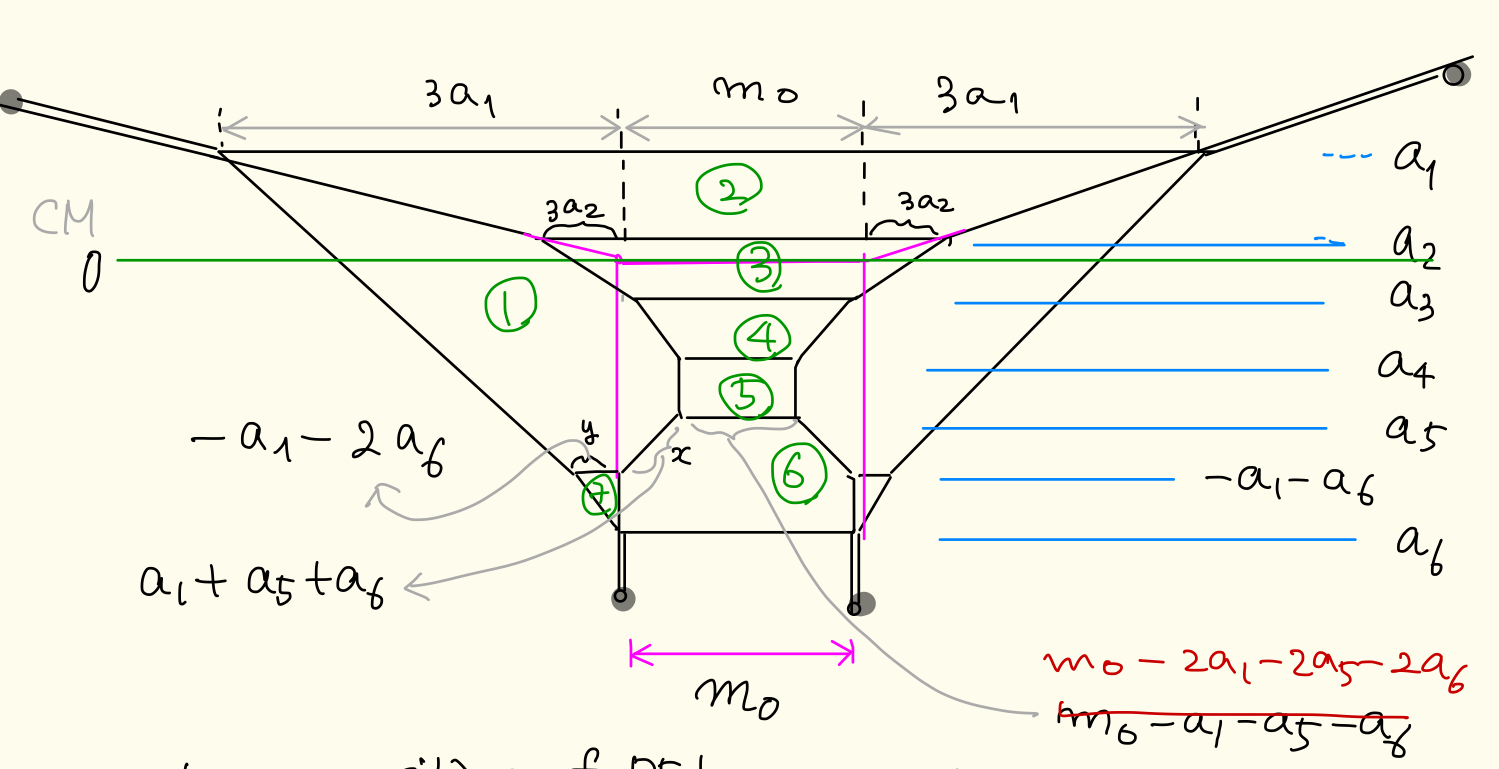
\includegraphics[width=10cm]{SU6-monopole.jpeg}
\caption{A 5-brane web for $SU(6)_3+1{\bf TAS}$ with massless ${\bf TAS}$.}
\label{fig:SU6-monopole}
\end{figure}
%----------------------------------%

  %---------  Figure  ---------------%
\begin{figure}[t]
\centering
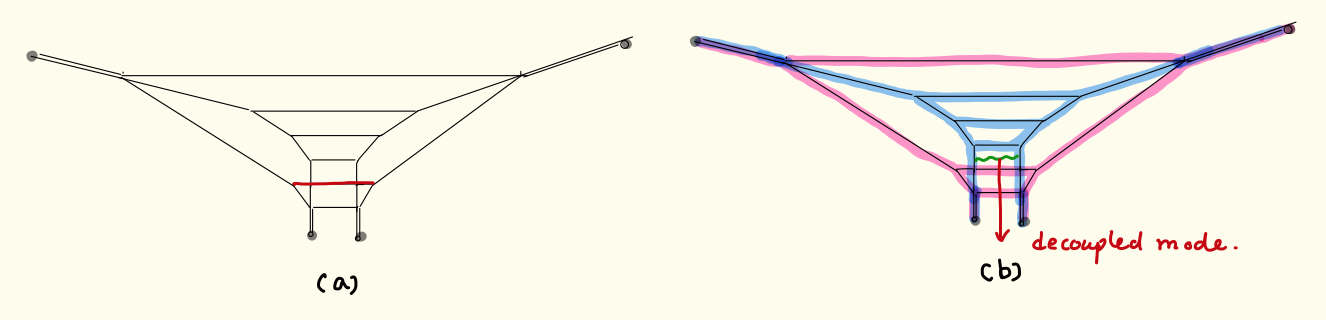
\includegraphics[width=12cm]{SU6-Higgsing.jpeg}
\caption{(a) A Higgsing from from $SU(6)_3+1{\bf TAS}$ to two $SU(3)_3$ theories. (a) Two $SU(3)_3$ theories are painted in blue and in pink respectively. A new decoupled mode emerges.}
\label{fig:SU6-Higgsing}
\end{figure}
%----------------------------------%

%---------  Figure  ---------------%
\begin{figure}[t]
\centering
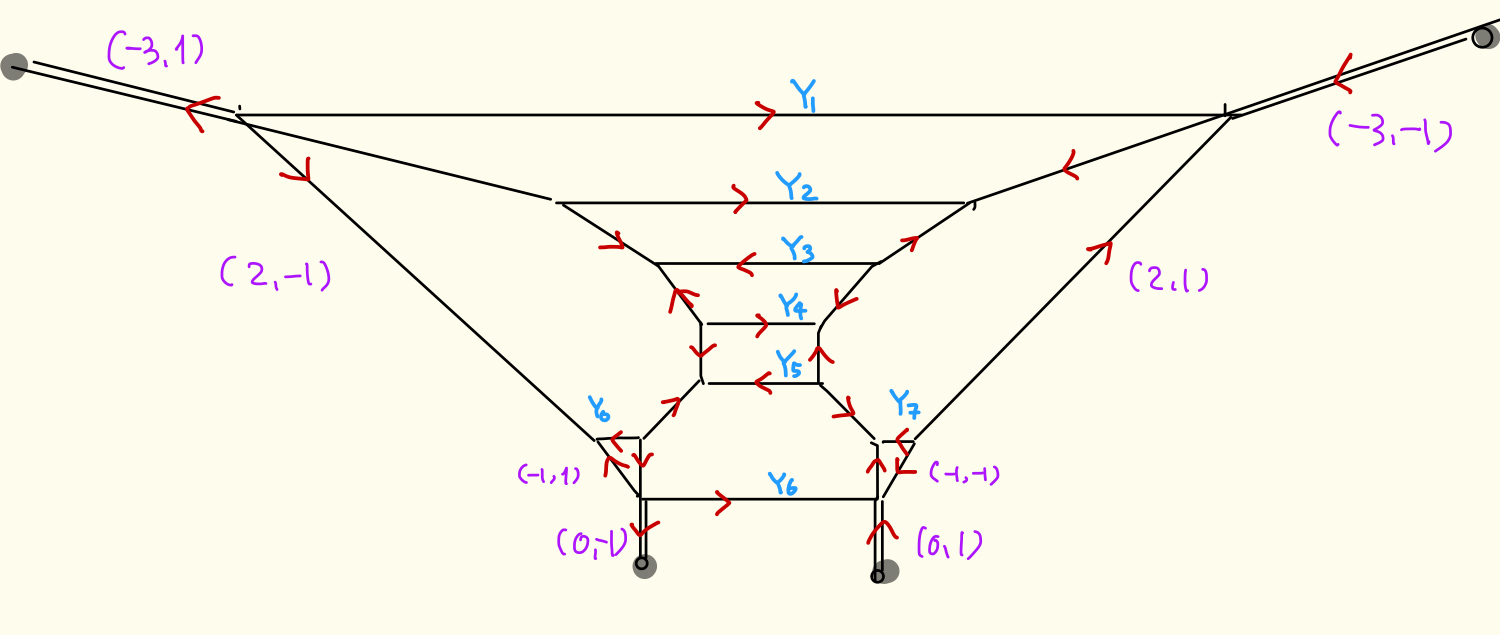
\includegraphics[width=10cm]{SU6young.jpeg}
\caption{A labeling of Young diagrams assigned to the horizontal lines in Figure \ref{fig:SU6-monopole}.}
\label{fig:SU6young}
\end{figure}
%----------------------------------%



\section{Conclusion} \label{sec:conclusion}


\acknowledgments
This work is supported in part by the UESTC Research Grant A03017023801317 (SSK), the National Research Foundation of Korea (NRF) Grants 2017R1D1A1B06034369 (KL, JS), and 2018R1A2B6004914 (KHL)


\bibliographystyle{JHEP}
\bibliography{ref}

\end{document}

